% Build with:  latexmk -pdf main.tex
% Needs a standard TeX Live installation (beamer, pgfplots, booktabs, lmodern, amsmath).
% Figures 2-4 are cropped from the paper and live in figs/ (fig2.png, fig3.png, fig4.png).
\documentclass[aspectratio=169,11pt]{beamer}

\usepackage[T1]{fontenc}
\usepackage[utf8]{inputenc}
\usepackage{lmodern}
\usepackage{amsmath,amssymb}
\usepackage{booktabs}
\usepackage{graphicx}
\usepackage{pgfplots}
\pgfplotsset{compat=1.16}

% ---------- look ----------
\definecolor{navy}{HTML}{14284B}
\definecolor{gold}{HTML}{9C7A2B}
\usetheme{default}
\setbeamertemplate{navigation symbols}{}
\setbeamercolor{structure}{fg=navy}
\setbeamercolor{frametitle}{fg=navy}
\setbeamercolor{title}{fg=navy}
\setbeamercolor{itemize item}{fg=gold}
\setbeamercolor{itemize subitem}{fg=gold}
\setbeamercolor{block title}{bg=navy!10,fg=navy}
\setbeamercolor{block body}{bg=navy!4}
\setbeamerfont{frametitle}{series=\bfseries,size=\Large}
\setbeamertemplate{itemize item}[square]
\setbeamertemplate{blocks}[default]
\setlength{\leftmargini}{1.2em}

% running header: set with \hdr{...} before each group of frames
\newcommand{\hdr}[1]{\gdef\curhdr{#1}}
\gdef\curhdr{}
\setbeamertemplate{headline}{%
  \leavevmode\hbox{\begin{beamercolorbox}[wd=\paperwidth,ht=3.2ex,dp=1.2ex,left]{headline}%
    \hspace*{1.1em}\scriptsize\textcolor{gray}{\textsc{\curhdr}}%
  \end{beamercolorbox}}\vskip-0.3ex\hrule height 0.5pt}
\setbeamertemplate{footline}{%
  \leavevmode\hbox{\begin{beamercolorbox}[wd=\paperwidth,ht=3ex,dp=1.4ex]{footline}%
    \hspace*{1.1em}\scriptsize\textcolor{gray}{COMP 599 \textperiodcentered{} Eliza Kishan\hfill
    Yang (2009), Firefly Algorithms for Multimodal Optimization\hfill
    \insertframenumber{} / \inserttotalframenumber\hspace*{1.1em}}%
  \end{beamercolorbox}}}

\newcommand{\Fig}[2]{\includegraphics[height=#1]{figs/#2}}

% ======================================================================
\begin{document}

% ---------------- title page ----------------
\begin{frame}[plain]
  \setbeamertemplate{headline}{}\setbeamertemplate{footline}{}
  \vspace*{0.6cm}
  {\color{gold}\rule{3cm}{2pt}}\par\vspace{0.4cm}
  {\color{navy}\fontsize{30}{34}\selectfont\bfseries Firefly Algorithms for\\Multimodal Optimization\par}
  \vspace{0.8cm}
  {\Large Xin-She Yang\par}
  \vspace{0.2cm}
  {\normalsize Department of Engineering, University of Cambridge\\
  Trumpington Street, Cambridge CB2 1PZ, UK\par}
  \vspace{0.5cm}
  {\small O.\ Watanabe and T.\ Zeugmann (Eds.): SAGA 2009, LNCS 5792, pp.\ 169--178, 2009.\\
  \copyright{} Springer-Verlag Berlin Heidelberg 2009\par}
  \vfill
  {\color{gold}\rule{\textwidth}{0.8pt}}\par\vspace{0.2cm}
  {\Large\itshape As presented by Eliza Kishan for COMP 599\par}
\end{frame}

% ---------------- abstract / outline ----------------
\hdr{Abstract}
\begin{frame}[t]{Abstract}
\begin{itemize}\itemsep0.6em
  \item Nature-inspired algorithms are among the most powerful algorithms for optimization.
  \item The paper gives a detailed description of a new \textbf{Firefly Algorithm (FA)} for multimodal optimization applications.
  \item FA is compared with other metaheuristic algorithms, in particular particle swarm optimization (PSO).
  \item Simulations and results indicate that the proposed firefly algorithm is superior to existing metaheuristic algorithms.
  \item The paper closes by discussing applications and implications for further research.
\end{itemize}
\end{frame}

\hdr{Outline}
\begin{frame}[t]{Outline: the paper's structure}
\begin{columns}[T]
\column{0.5\textwidth}
\begin{enumerate}\setlength{\itemsep}{0.5em}
  \item[\textbf{1}] Introduction
  \item[\textbf{2}] Particle Swarm Optimization
    \begin{itemize}\item[] 2.1 Standard PSO\end{itemize}
  \item[\textbf{3}] Firefly Algorithm
    \begin{itemize}\item[] 3.1 Behaviour of Fireflies
      \item[] 3.2 Firefly Algorithm
      \item[] 3.3 Attractiveness
      \item[] 3.4 Distance and Movement
      \item[] 3.5 Scaling and Asymptotic Cases\end{itemize}
\end{enumerate}
\column{0.5\textwidth}
\begin{enumerate}\setlength{\itemsep}{0.5em}
  \item[\textbf{4}] Multimodal Optimization with Multiple Optima
    \begin{itemize}\item[] 4.1 Validation
      \item[] 4.2 Comparison of FA with PSO and GA\end{itemize}
  \item[\textbf{5}] Conclusions
  \item[] References, followed by discussion points
\end{enumerate}
\begin{block}{Source}\small
X.-S. Yang, ``Firefly Algorithms for Multimodal Optimization,'' in O.\ Watanabe and T.\ Zeugmann (Eds.), \emph{SAGA 2009}, LNCS 5792, pp.\ 169--178. Springer, Berlin Heidelberg (2009).
\end{block}
\end{columns}
\end{frame}

% ---------------- 1 Introduction ----------------
\hdr{1 Introduction}
\begin{frame}[t]{Introduction: biologically inspired optimization}
\begin{itemize}\itemsep0.7em
  \item Biologically inspired algorithms are becoming powerful in modern numerical optimization [1, 2, 4, 6, 9, 10], especially for \textbf{NP-hard} problems such as the travelling salesman problem.
  \item Among these biology-derived algorithms, \textbf{multi-agent metaheuristics} such as particle swarm optimization are hot research topics in state-of-the-art algorithm development, in optimization and other applications [1, 2, 9].
  \item \textbf{PSO} was developed by Kennedy and Eberhart in 1995 [5], based on swarm behaviour such as fish and bird schooling in nature: so-called \emph{swarm intelligence}.
\end{itemize}
\end{frame}

\begin{frame}[t]{Introduction: PSO compared with genetic algorithms}
\begin{itemize}\itemsep0.7em
  \item PSO has many similarities with genetic algorithms (GA), but it is much simpler.
  \item It uses \textbf{no mutation or crossover operators}.
  \item Instead it uses real-number randomness and global communication among the swarming particles.
  \item In this sense it is also easier to implement, since it mainly uses real numbers.
\end{itemize}
\end{frame}

\begin{frame}[t]{Introduction: aims and claims of the paper}
\begin{itemize}\itemsep0.7em
  \item \textbf{Aim:} introduce the new Firefly Algorithm and provide a comparison study of FA with PSO and other relevant algorithms.
  \item \textbf{Plan:} first outline particle swarm optimization, then formulate the firefly algorithm, and finally compare the performance of these algorithms.
  \item \textbf{Claim 1:} FA seems more promising than PSO, because it can deal with \textbf{multimodal functions} more naturally and efficiently.
  \item \textbf{Claim 2:} PSO is just a special class of firefly algorithms, as the paper demonstrates.
\end{itemize}
\end{frame}

% ---------------- 2 PSO ----------------
\hdr{2 Particle Swarm Optimization \textperiodcentered{} 2.1 Standard PSO}
\begin{frame}[t]{Standard PSO: how the swarm searches}
\small
\begin{itemize}\itemsep0.45em
  \item PSO searches the space of the objective function by adjusting the trajectories of individual agents, called \textbf{particles}: piecewise paths formed by positional vectors, in a quasi-stochastic manner [5, 6].
  \item There are about 20 different variants of PSO; the paper describes only the simplest and yet popular \textbf{standard PSO}.
  \item Particle movement has two components: a \textbf{stochastic} component and a \textbf{deterministic} component.
  \item A particle is attracted toward the current global best $g^*$ and its own best location $x_i^*$ in history, while also tending to move randomly.
  \item When a particle finds a location better than any previously found, it becomes the new current best for particle $i$; there is one current global best for all $n$ particles.
  \item The aim is to find the global best among all current bests, until the objective no longer improves or after a fixed number of iterations.
\end{itemize}
\end{frame}

\begin{frame}[t]{Standard PSO: velocity and position updates}
\small
$x_i^*$ is the current best for particle $i$, and $g^*\approx\min\text{ or }\max\{f(x_i)\}$ $(i=1,2,\dots,n)$ the current global best. $x_i$ and $v_i$ are the position and velocity vectors of particle $i$.
\begin{align*}
v_i^{t+1}&=v_i^{t}+\alpha\,\epsilon_1\odot(g^*-x_i^t)+\beta\,\epsilon_2\odot(x_i^*-x_i^t)\tag{1}\\
x_i^{t+1}&=x_i^{t}+v_i^{t+1}\tag{2}
\end{align*}
\begin{itemize}\itemsep0.3em
  \item $\epsilon_1$ and $\epsilon_2$ are random vectors, each entry between 0 and 1.
  \item The \textbf{Hadamard product} is the entrywise product: $[u\odot v]_{ij}=u_{ij}v_{ij}$.
  \item $\alpha$ and $\beta$ are learning parameters (acceleration constants), typically $\alpha\approx\beta\approx 2$.
  \item Initial values: $x_i^{t=0}$ taken within the bounds $a=\min(x_j)$, $b=\max(x_j)$, and $v_i^{t=0}=0$. The velocity is usually bounded to a range $[0,v_{\max}]$.
\end{itemize}
\end{frame}

\begin{frame}[t]{Standard PSO: variants and the inertia function}
\begin{itemize}\itemsep0.5em
  \item Many variants extend standard PSO; the most noticeable improvement is probably the \textbf{inertia function} $\theta(t)$.
  \item $v_i^t$ is replaced by $\theta(t)\,v_i^t$, where $\theta$ takes values between 0 and 1.
  \item In the simplest case the inertia function is a constant, typically $\theta\approx 0.5\sim 0.9$.
  \item This is equivalent to introducing a \textbf{virtual mass} that stabilizes the motion of the particles, so the algorithm is expected to converge more quickly.
\end{itemize}
\[v_i^{t+1}=\theta(t)\,v_i^{t}+\alpha\,\epsilon_1\odot(g^*-x_i^t)+\beta\,\epsilon_2\odot(x_i^*-x_i^t)\]
{\footnotesize\itshape Written out from the text's description; the paper gives no separate equation number for it. The comparison in \S4.2 uses PSO without this correction.\par}
\end{frame}

% ---------------- 3 Firefly algorithm ----------------
\hdr{3 Firefly Algorithm \textperiodcentered{} 3.1 Behaviour of Fireflies}
\begin{frame}[t]{Behaviour of fireflies: the flashing signal}
\begin{itemize}\itemsep0.7em
  \item The flashing light of fireflies is an amazing sight in the summer sky in tropical and temperate regions.
  \item There are about \textbf{two thousand} firefly species, and most produce short, rhythmic flashes; the pattern of flashes is often unique to a particular species.
  \item The light is produced by \textbf{bioluminescence}, and the true functions of such signalling systems are still debated.
  \item Two fundamental functions: to \textbf{attract mating partners} (communication) and to \textbf{attract potential prey}. Flashing may also serve as a protective warning mechanism.
\end{itemize}
\end{frame}

\begin{frame}[t]{Behaviour of fireflies: a signal system}
\begin{itemize}\itemsep0.8em
  \item The rhythm of the flash, the rate of flashing and the amount of time form part of the signal system that brings both sexes together.
  \item Females respond to a male's unique flashing pattern within the same species.
  \item In some species such as \emph{Photuris}, female fireflies can \textbf{mimic the mating flash pattern of other species} so as to lure and eat the male fireflies, who mistake the flashes for a suitable mate.
\end{itemize}
\end{frame}

\begin{frame}[t]{Behaviour of fireflies: light intensity and distance}
\begin{itemize}\itemsep0.5em
  \item Light intensity at distance $r$ from the source obeys the \textbf{inverse square law}: intensity $I$ decreases as $r$ increases, $I\propto 1/r^2$.
  \item In addition, the air \textbf{absorbs} light, which becomes weaker and weaker with distance.
  \item These two factors combined make most fireflies visible only to a limited distance, usually several hundred metres at night, which is enough for them to communicate.
  \item The flashing light can be formulated so that it is associated with the \textbf{objective function} to be optimized, which makes new optimization algorithms possible.
\end{itemize}
\[I\propto\frac{1}{r^{2}}\]
{\footnotesize\itshape The paper next outlines the basic formulation of FA, then discusses implementation and analysis in detail.\par}
\end{frame}

\hdr{3 Firefly Algorithm \textperiodcentered{} 3.2 Firefly Algorithm}
\begin{frame}[t]{Firefly algorithm: three idealized rules}
\begin{enumerate}\itemsep0.8em
  \item All fireflies are \textbf{unisex}, so one firefly is attracted to other fireflies regardless of their sex.
  \item \textbf{Attractiveness is proportional to brightness}: of any two flashing fireflies, the less bright one moves towards the brighter one. Attractiveness and brightness both decrease as distance increases. If no firefly is brighter than a particular firefly, it moves randomly.
  \item The \textbf{brightness} of a firefly is affected or determined by the landscape of the objective function. For a maximization problem, brightness can simply be proportional to the objective value. Other forms of brightness can be defined like a fitness function in genetic algorithms.
\end{enumerate}
{\small\itshape Based on these three rules, the basic steps of the algorithm are summarized as the pseudo code in Fig.~1.\par}
\end{frame}

\begin{frame}[t]{Firefly algorithm: pseudo code (Fig.\ 1)}
\begin{columns}[T]
\column{0.58\textwidth}
\footnotesize
\hrule\vspace{0.4em}
\noindent\textbf{Firefly Algorithm}\par
Objective function $f(\mathbf{x})$, $\mathbf{x}=(x_1,\dots,x_d)^T$\par
Generate initial population of fireflies $x_i$ $(i=1,2,\dots,n)$\par
Light intensity $I_i$ at $x_i$ is determined by $f(x_i)$\par
Define light absorption coefficient $\gamma$\par
\textbf{while} ($t<$ MaxGeneration)\par
\hspace*{1em}\textbf{for} $i=1:n$ all $n$ fireflies\par
\hspace*{2em}\textbf{for} $j=1:i$ all $n$ fireflies\par
\hspace*{3em}\textbf{if} ($I_j>I_i$), move firefly $i$ towards $j$ in $d$-dimension; \textbf{end if}\par
\hspace*{3em}Attractiveness varies with distance $r$ via $\exp[-\gamma r]$\par
\hspace*{3em}Evaluate new solutions and update light intensity\par
\hspace*{2em}\textbf{end for} $j$\par
\hspace*{1em}\textbf{end for} $i$\par
\hspace*{1em}Rank the fireflies and find the current best\par
\textbf{end while}\par
Postprocess results and visualization\par
\vspace{0.3em}\hrule
\column{0.4\textwidth}
{\footnotesize\textbf{Fig.\ 1.} Pseudo code of the firefly algorithm (FA), typeset from the paper.\par}
\vspace{0.5em}
\begin{block}{Reading the pseudo code}\footnotesize
\begin{itemize}\itemsep0.2em
  \item Each firefly is compared with the others; a dimmer firefly moves toward a brighter one.
  \item As printed, the attractiveness in Fig.~1 decays as $\exp[-\gamma r]$, whereas Eq.~(6) uses $\exp(-\gamma r^2)$.
  \item The inner loop runs over all fireflies, so each generation compares pairs of fireflies.
\end{itemize}
\end{block}
\end{columns}
\end{frame}

\begin{frame}[t]{Firefly algorithm: relation to bacterial foraging}
\begin{itemize}\itemsep0.8em
  \item There is some conceptual similarity between the firefly algorithm and the \textbf{bacterial foraging algorithm (BFA)} [3, 7].
  \item In BFA, the attraction among bacteria is based partly on their fitness and partly on their distance.
  \item In FA, the attractiveness is linked to the objective function and decays monotonically with distance.
  \item The agents in FA have \textbf{adjustable visibility} and more versatile attractiveness variations, which usually leads to higher mobility, so the search space is explored more efficiently.
\end{itemize}
\end{frame}

\hdr{3 Firefly Algorithm \textperiodcentered{} 3.3 Attractiveness}
\begin{frame}[t]{Attractiveness: brightness and the eye of the beholder}
\begin{itemize}\itemsep0.6em
  \item Two important issues: the \textbf{variation of light intensity} and the \textbf{formulation of the attractiveness}.
  \item For simplicity, the attractiveness of a firefly is determined by its brightness, which in turn is associated with the encoded objective function.
  \item In the simplest case for maximization problems, the brightness $I$ of a firefly at location $x$ can be chosen as $I(x)\propto f(x)$.
  \item The attractiveness $\beta$ is \textbf{relative}: it is seen in the eyes of the beholder, judged by the other fireflies, so it varies with the distance $r_{ij}$ between firefly $i$ and firefly $j$.
  \item Light intensity decreases with distance from its source and light is absorbed in the medium, so attractiveness should vary with the degree of absorption.
\end{itemize}
\end{frame}

\begin{frame}[t]{Attractiveness: from inverse-square decay to a Gaussian}
\small
In the simplest form, intensity follows the inverse square law, with $I_s$ the intensity at the source:
\[I(r)=\frac{I_s}{r^{2}}\]
For a medium with fixed light absorption coefficient $\gamma$, the intensity varies with distance as
\[I=I_0\,e^{-\gamma r}\]
with $I_0$ the original intensity. To avoid the singularity at $r=0$ in $I_s/r^2$, the combined effect of the inverse square law and absorption is approximated by a Gaussian form:
\begin{equation*}I(r)=I_0\,e^{-\gamma r^{2}}\tag{3}\end{equation*}
When a slower monotonic decrease is needed, the following approximation can be used:
\begin{equation*}I(r)=\frac{I_0}{1+\gamma r^{2}}\tag{4}\end{equation*}
\end{frame}

\begin{frame}[t]{Attractiveness: $\beta(r)$ and the characteristic distance}
\small
At short distance the two forms are essentially the same, because their series expansions about $r=0$ agree up to the order $O(r^3)$:
\begin{equation*}e^{-\gamma r^{2}}\approx 1-\gamma r^{2}+\tfrac12\gamma^{2}r^{4}+\dots,\qquad \frac{1}{1+\gamma r^{2}}\approx 1-\gamma r^{2}+\gamma^{2}r^{4}+\dots\tag{5}\end{equation*}
Since attractiveness is proportional to the light intensity seen by adjacent fireflies, define
\begin{equation*}\beta(r)=\beta_0\,e^{-\gamma r^{2}}\tag{6}\end{equation*}
where $\beta_0$ is the attractiveness at $r=0$. Because $1/(1+r^2)$ is often faster to compute than an exponential, the form below can replace it if necessary:
\[\beta=\frac{\beta_0}{1+\gamma r^{2}}\]
Eq.~(6) defines a \textbf{characteristic distance} $\Gamma=1/\sqrt{\gamma}$ over which the attractiveness changes significantly from $\beta_0$ to $\beta_0 e^{-1}$.
\end{frame}

\begin{frame}[t]{Attractiveness: the generalized form}
In an implementation, the attractiveness function $\beta(r)$ can be any monotonically decreasing function, such as the generalized form
\begin{equation*}\beta(r)=\beta_0\,e^{-\gamma r^{m}}\qquad(m\ge 1)\tag{7}\end{equation*}
\begin{itemize}\itemsep0.5em
  \item For a fixed $\gamma$, the characteristic length becomes $\Gamma=\gamma^{-1/m}\to 1$ as $m\to\infty$.
  \item Conversely, for a given length scale $\Gamma$ in an optimization problem, $\gamma$ can be used as a typical initial value:
\end{itemize}
\[\gamma=\frac{1}{\Gamma^{m}}\]
\end{frame}

\hdr{3 Firefly Algorithm \textperiodcentered{} 3.4 Distance and Movement}
\begin{frame}[t]{Distance and movement: the update equation}
\small
The distance between fireflies $i$ and $j$ at $x_i$ and $x_j$ is the Cartesian distance
\begin{equation*}r_{ij}=\lVert x_i-x_j\rVert=\sqrt{\sum_{k=1}^{d}(x_{i,k}-x_{j,k})^{2}}\tag{8}\end{equation*}
where $x_{i,k}$ is the $k$th component of the spatial coordinate $x_i$ of firefly $i$. In the 2-D case:
\[r_{ij}=\sqrt{(x_i-x_j)^2+(y_i-y_j)^2}\]
The movement of firefly $i$, attracted to a more attractive (brighter) firefly $j$, is determined by
\begin{equation*}x_i=x_i+\beta_0\,e^{-\gamma r_{ij}^{2}}(x_j-x_i)+\alpha\left(\mathrm{rand}-\tfrac12\right)\tag{9}\end{equation*}
The second term is due to the attraction; the third is randomization, with $\alpha$ the randomization parameter and $\mathrm{rand}$ a random number generator uniformly distributed in $[0,1]$.
\end{frame}

\begin{frame}[t]{Distance and movement: parameter choices}
\small
\begin{itemize}\itemsep0.6em
  \item For most cases in the implementation, take $\beta_0=1$ and $\alpha\in[0,1]$.
  \item The randomization term can easily be extended to a \textbf{normal distribution} $N(0,1)$ or other distributions.
  \item If scales differ significantly between dimensions, for example $-10^5$ to $10^5$ in one dimension but about $-0.001$ to $0.01$ along another, replace $\alpha$ by $\alpha S_k$, where the scaling parameters $S_k$ $(k=1,\dots,d)$ follow the actual scales of the problem.
  \item $\gamma$ characterizes the variation of the attractiveness; its value is crucially important in determining the \textbf{speed of convergence} and how FA behaves.
  \item In theory $\gamma\in[0,\infty)$; in practice $\gamma=O(1)$, determined by the characteristic length $\Gamma$ of the system, and typically varies from 0.01 to 100.
\end{itemize}
\end{frame}

\hdr{3 Firefly Algorithm \textperiodcentered{} 3.5 Scaling and Asymptotic Cases}
\begin{frame}[t]{Scaling: the distance $r$ is not limited to Euclidean}
\begin{itemize}\itemsep0.6em
  \item Many other forms of distance $r$ can be defined in the $n$-dimensional hyperspace, depending on the problem of interest.
  \item \textbf{Job scheduling:} $r$ can be defined as the time lag or time interval.
  \item \textbf{Complicated networks} such as the Internet and social networks: $r$ can combine the degree of local clustering and the average proximity of vertices.
  \item In fact, any measure that effectively characterizes the quantities of interest in the optimization problem can be used as the ``distance'' $r$.
  \item The typical scale $\Gamma$ should be associated with the scale of the optimization problem of interest.
\end{itemize}
\end{frame}

\begin{frame}[t]{Scaling: many fireflies and many local optima}
\small
\begin{itemize}\itemsep0.55em
  \item Let $\Gamma$ be the typical scale of a problem, and take a very large number of fireflies, $n\gg m$, where $m$ is the number of \textbf{local optima}.
  \item The initial locations should then be distributed relatively uniformly over the entire search space, as in the initialization of \textbf{quasi-Monte Carlo} simulations.
  \item As iterations proceed, the fireflies converge into \textbf{all the local optima} (including the global ones) in a stochastic manner. Comparing the best solutions among these optima gives the global optimum.
  \item The author is trying to prove formally that FA approaches the global optima when $n\to\infty$ and $t\gg 1$.
  \item In reality it converges very quickly, typically in \textbf{fewer than 50 to 100 generations}, demonstrated later on standard test functions.
\end{itemize}
\end{frame}

\begin{frame}[t]{Scaling: the limits $\gamma\to 0$ and $\gamma\to\infty$}
\small
\begin{columns}[T]
\column{0.49\textwidth}
\begin{block}{$\gamma\to 0$}
\begin{itemize}\itemsep0.3em
  \item Attractiveness is constant, $\beta=\beta_0$, and $\Gamma\to\infty$.
  \item Light intensity does not decrease in an idealized sky, so a flashing firefly can be seen anywhere in the domain.
  \item A single (usually global) optimum can easily be reached.
  \item This corresponds to a special case of PSO, with the same efficiency as PSO.
\end{itemize}
\end{block}
\column{0.49\textwidth}
\begin{block}{$\gamma\to\infty$}
\begin{itemize}\itemsep0.3em
  \item $\Gamma\to 0$ and $\beta(r)\to\delta(r)$, the Dirac delta function.
  \item Attractiveness is almost zero in the sight of other fireflies: they are short-sighted, as if flying randomly in a very foggy region.
  \item No other firefly can be seen, and each roams in a completely random way.
  \item This corresponds to the completely random search method.
\end{itemize}
\end{block}
\end{columns}
\end{frame}

\begin{frame}[t]{Scaling: between the two extremes}
\begin{itemize}\itemsep0.7em
  \item FA usually lies somewhere between these two extremes, so $\gamma$ and $\alpha$ can be adjusted to \textbf{outperform both random search and PSO}.
  \item In fact FA can find the \textbf{global optima as well as all the local optima simultaneously} in a very effective manner; this is demonstrated later.
  \item Different fireflies work almost independently, so FA is particularly suitable for \textbf{parallel implementation}.
  \item It is even better than genetic algorithms and PSO, because fireflies \textbf{aggregate more closely} around each optimum, without jumping around as in genetic algorithms.
  \item The interactions between different subregions are minimal in a parallel implementation.
\end{itemize}
\end{frame}

% ---------------- 4 Multimodal optimization ----------------
\hdr{4 Multimodal Optimization with Multiple Optima \textperiodcentered{} 4.1 Validation}
\begin{frame}[t]{Validation: the Michalewicz function}
\small
To demonstrate how FA works, the author implemented it in \textbf{Matlab} and validated it on various test functions. First example, the Michalewicz function:
\begin{equation*}f(\mathbf{x})=-\sum_{i=1}^{d}\sin(x_i)\left[\sin\!\left(\frac{i\,x_i^{2}}{\pi}\right)\right]^{2m}\tag{10}\end{equation*}
\begin{itemize}\itemsep0.3em
  \item $m=10$ and $d=1,2,\dots$
  \item The global minimum $f_*\approx-1.801$ in 2-D occurs at $(2.20319,\,1.57049)$.
  \item FA finds it after about \textbf{400 evaluations} for \textbf{40 fireflies} after \textbf{10 iterations} (Figs.~2 and 3).
  \item Parameter values in these simulations: $\alpha=0.2$, $\gamma=1$, $\beta_0=1$.
  \item The paper calls this much more efficient than most existing metaheuristic algorithms, and goes on to tougher test functions.
\end{itemize}
\end{frame}

\begin{frame}[t]{Validation: Michalewicz's function in 2-D (Fig.\ 2)}
\centering
\Fig{0.62\textheight}{fig2.png}\par\vspace{0.4em}
{\small\textbf{Fig.\ 2.} Michalewicz's function for two independent variables with a global minimum $f_*\approx-1.801$ at $(2.20319,\,1.57049)$. Reproduced from the paper.\par}
\end{frame}

\begin{frame}[t]{Validation: initial and final firefly positions (Fig.\ 3)}
\centering
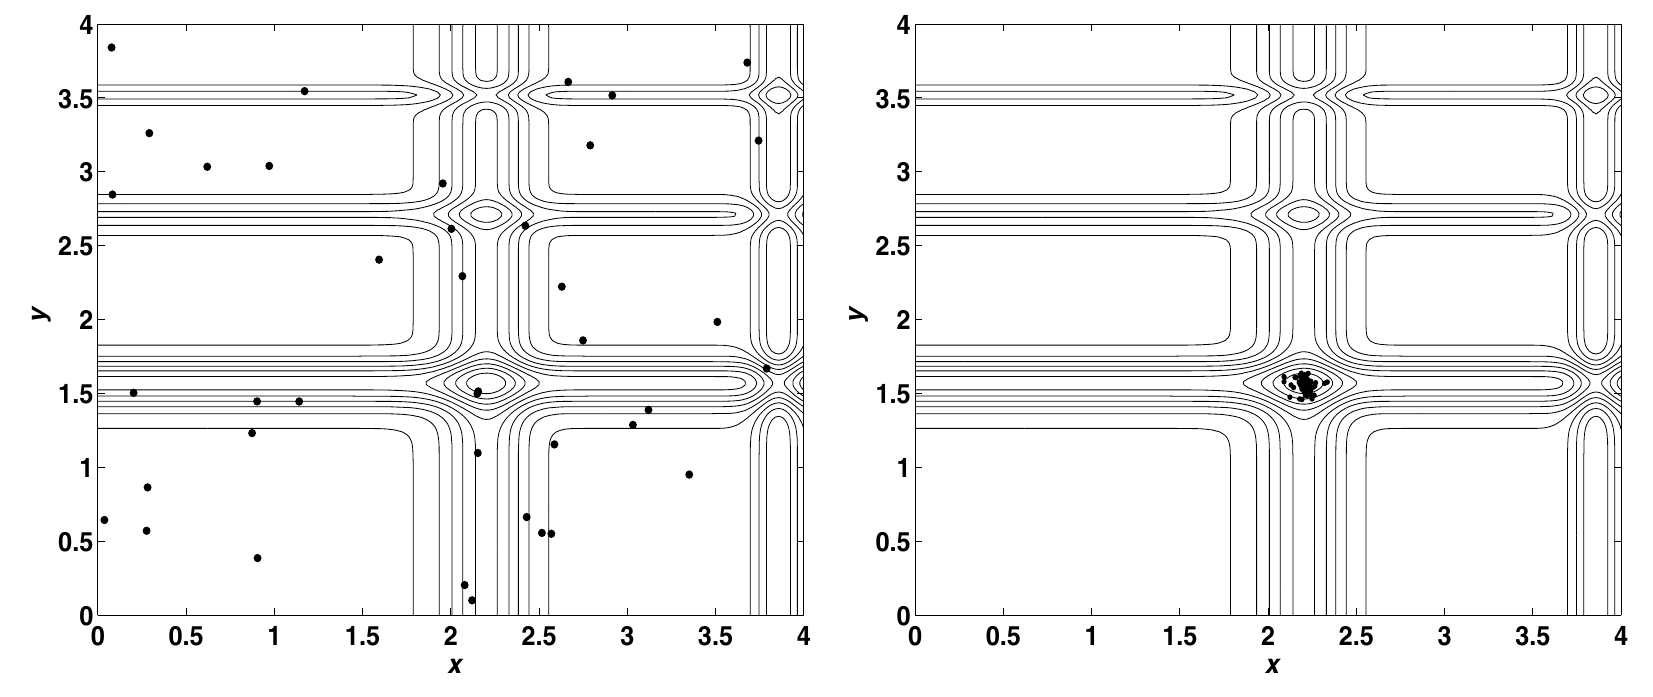
\includegraphics[height=0.52\textheight]{figs/fig3.png}\par\vspace{0.4em}
{\small\textbf{Fig.\ 3.} The initial 40 fireflies (left) and their locations after 10 iterations (right). Reproduced from the paper.\par}
\vspace{0.3em}
{\small\itshape After 10 iterations the swarm has clustered at the global minimum near $(2.2,\,1.57)$ of the contour plot.\par}
\end{frame}

\begin{frame}[t]{Validation: Yang's standing-wave function}
\small
A much tougher test function, described by Yang [11], looks like a standing-wave pattern:
\begin{equation*}f(\mathbf{x})=\left[e^{-\sum_{i=1}^{d}(x_i/a)^{2m}}-2e^{-\sum_{i=1}^{d}x_i^{2}}\right]\cdot\prod_{i=1}^{d}\cos^{2}x_i,\qquad m=5\tag{11}\end{equation*}
\begin{columns}[T]
\column{0.5\textwidth}
\begin{itemize}\itemsep0.4em
  \item Multimodal, with many local peaks and valleys.
  \item A unique global minimum $f_*=-1$ at $(0,0,\dots,0)$ in the region $-20\le x_i\le 20$, $i=1,2,\dots,d$, with $a=15$.
  \item The 2-D landscape is shown in Fig.~4.
\end{itemize}
\column{0.5\textwidth}
\centering
\Fig{0.38\textheight}{fig4.png}\par
{\footnotesize\textbf{Fig.\ 4.} Yang's function in 2D with a global minimum $f_*=-1$ at $(0,0)$ where $a=15$. Reproduced from the paper.\par}
\end{columns}
\end{frame}

\hdr{4 Multimodal Optimization with Multiple Optima \textperiodcentered{} 4.2 Comparison of FA with PSO and GA}
\begin{frame}[t]{Comparison: rationale}
\begin{itemize}\itemsep0.8em
  \item Various studies show that PSO can outperform genetic algorithms (GA) [4] and other conventional algorithms on many optimization problems.
  \item This is partly because broadcasting the current best estimates gives better and quicker convergence towards the optimum.
  \item A general framework for evaluating the statistical performance of evolutionary algorithms has been discussed in detail by Shilane et al. [8].
  \item The paper now compares the firefly algorithm with PSO and with genetic algorithms on various standard test functions.
\end{itemize}
\end{frame}

\begin{frame}[t]{Comparison: algorithm settings}
\begin{center}\small
\begin{tabular}{@{}p{0.12\textwidth}p{0.82\textwidth}@{}}
\toprule
\textbf{Algorithm} & \textbf{Version and parameters used}\\\midrule
GA  & Standard version with \textbf{no elitism}; mutation probability $p_m=0.05$; crossover probability $0.95$.\\[0.4em]
PSO & Standard version; learning parameters $\alpha\approx\beta\approx2$; \textbf{without the inertia correction} [4, 5, 6].\\[0.4em]
FA  & $\alpha=0.2$, $\gamma=1$, $\beta_0=1$, as stated for the validation simulations of \S4.1; the comparison itself does not restate them.\\
\bottomrule
\end{tabular}
\end{center}
\vspace{0.6em}
\textbf{Population size.} Sizes from $n=15$ to $200$ were tried; for most problems $n=15$ to $50$ is sufficient. A fixed \textbf{$n=40$} was therefore used in all comparison simulations.
\end{frame}

\begin{frame}[t]{Comparison: simulation protocol}
\begin{itemize}\itemsep0.7em
  \item All three algorithms were implemented in \textbf{Matlab}, followed by extensive simulations.
  \item Each algorithm was run \textbf{at least 100 times}, so as to carry out meaningful statistical analysis.
  \item The algorithms stop when the variation of function values is less than a given tolerance $\epsilon\le10^{-5}$.
  \item Table 1 summarizes the cases where the global optima are reached. Format: \textbf{average number of evaluations $\pm$ standard deviation (success rate)}.
  \item Example: $3752\pm725\,(99\%)$ means a mean of 3752 function evaluations with standard deviation 725, and a success rate of 99\% in finding the global optimum.
\end{itemize}
\end{frame}

\begin{frame}[t]{Test functions used in Table 1 (1/2)}
\scriptsize
\renewcommand{\arraystretch}{1.25}\setlength{\tabcolsep}{3pt}
\begin{tabular}{@{}p{0.12\textwidth}p{0.50\textwidth}p{0.29\textwidth}@{}}
\toprule
\textbf{Function} & \textbf{Formula} & \textbf{Domain, optimum, citation}\\\midrule
Michalewicz & $\displaystyle f(\mathbf{x})=-\sum_{i=1}^{d}\sin(x_i)\Big[\sin\!\Big(\tfrac{i\,x_i^{2}}{\pi}\Big)\Big]^{2m},\ m=10$ & $0\le x_i\le\pi$; $f_*\approx-1.801$ in 2-D. Paper Eq.~(10) [12]\\
Rosenbrock & $\displaystyle f(\mathbf{x})=\sum_{i=1}^{d-1}\big[100(x_{i+1}-x_i^{2})^{2}+(x_i-1)^{2}\big]$ & $-30\le x_i\le30$; $f_*=0$ at $(1,\dots,1)$. [13]\\
De Jong (sphere) & $\displaystyle f(\mathbf{x})=\sum_{i=1}^{d}x_i^{2}$ & $-5.12\le x_i\le5.12$; $f_*=0$ at $\mathbf{0}$. [14]\\
Schwefel & $\displaystyle f(\mathbf{x})=-\sum_{i=1}^{d}x_i\sin\!\big(\sqrt{|x_i|}\big)$ & $-500\le x_i\le500$; $f_*\approx-418.983\,d$. [15]\\
Ackley & $\displaystyle f(\mathbf{x})=-20e^{-0.2\sqrt{\frac1d\sum_{i}x_i^{2}}}-e^{\frac1d\sum_{i}\cos(2\pi x_i)}+20+e$ & $-32.768\le x_i\le32.768$; $f_*=0$ at $\mathbf{0}$. [16]\\
\bottomrule
\end{tabular}
\end{frame}

\begin{frame}[t]{Test functions used in Table 1 (2/2)}
\scriptsize
\renewcommand{\arraystretch}{1.25}\setlength{\tabcolsep}{3pt}
\begin{tabular}{@{}p{0.12\textwidth}p{0.50\textwidth}p{0.29\textwidth}@{}}
\toprule
\textbf{Function} & \textbf{Formula} & \textbf{Domain, optimum, citation}\\\midrule
Rastrigin & $\displaystyle f(\mathbf{x})=10d+\sum_{i=1}^{d}\big[x_i^{2}-10\cos(2\pi x_i)\big]$ & $-5.12\le x_i\le5.12$; $f_*=0$ at $\mathbf{0}$. [17]\\
Easom & $\displaystyle f(\mathbf{x})=-\cos(x_1)\cos(x_2)\,e^{-(x_1-\pi)^{2}-(x_2-\pi)^{2}}$ & $-100\le x_i\le100$; $f_*=-1$ at $(\pi,\pi)$. [18]\\
Griewank & $\displaystyle f(\mathbf{x})=\frac{1}{4000}\sum_{i=1}^{d}x_i^{2}-\prod_{i=1}^{d}\cos\!\Big(\tfrac{x_i}{\sqrt i}\Big)+1$ & $-600\le x_i\le600$; $f_*=0$ at $\mathbf{0}$. [19]\\
Shubert & $\displaystyle f(\mathbf{x})=\prod_{i=1}^{d}\Big[\sum_{j=1}^{5}\cos\big((j+1)x_i+j\big)\Big]$ & $-10\le x_i\le10$; 18 global minima in 2-D, $f_*\approx-186.73$. [20]\\
Yang & $\displaystyle f(\mathbf{x})=\Big[e^{-\sum_i(x_i/a)^{2m}}-2e^{-\sum_i x_i^{2}}\Big]\prod_i\cos^{2}x_i$ & $m=5$, $a=15$, $-20\le x_i\le20$; $f_*=-1$ at $\mathbf{0}$. Paper Eq.~(11) [11]\\
\bottomrule
\end{tabular}
\par\vspace{0.2em}
{\scriptsize\itshape Only the Michalewicz and Yang formulas are given in the paper. The others are the standard literature forms; the author's exact parameters may differ.\par}
\end{frame}

\begin{frame}[t]{Table 1. Comparison of algorithm performance}
\centering\small\setlength{\tabcolsep}{3pt}
\begin{tabular}{lccc}
\toprule
\textbf{Functions / Algorithms} & \textbf{GA} & \textbf{PSO} & \textbf{FA}\\\midrule
Michalewicz's ($d=16$) & $89325\pm7914$ (95\%) & $6922\pm537$ (98\%) & $3752\pm725$ (99\%)\\
Rosenbrock's ($d=16$) & $55723\pm8901$ (90\%) & $32756\pm5325$ (98\%) & $7792\pm2923$ (99\%)\\
De Jong's ($d=256$) & $25412\pm1237$ (100\%) & $17040\pm1123$ (100\%) & $7217\pm730$ (100\%)\\
Schwefel's ($d=128$) & $227329\pm7572$ (95\%) & $14522\pm1275$ (97\%) & $9902\pm592$ (100\%)\\
Ackley's ($d=128$) & $32720\pm3327$ (90\%) & $23407\pm4325$ (92\%) & $5293\pm4920$ (100\%)\\
Rastrigin's & $110523\pm5199$ (77\%) & $79491\pm3715$ (90\%) & $15573\pm4399$ (100\%)\\
Easom's & $19239\pm3307$ (92\%) & $17273\pm2929$ (90\%) & $7925\pm1799$ (100\%)\\
Griewank's & $70925\pm7652$ (90\%) & $55970\pm4223$ (92\%) & $12592\pm3715$ (100\%)\\
Shubert's (18 minima) & $54077\pm4997$ (89\%) & $23992\pm3755$ (92\%) & $12577\pm2356$ (100\%)\\
Yang's ($d=16$) & $27923\pm3025$ (83\%) & $14116\pm2949$ (90\%) & $7390\pm2189$ (100\%)\\
\bottomrule
\end{tabular}\par\vspace{0.2em}
{\footnotesize\itshape Entries: mean number of function evaluations $\pm$ standard deviation (success rate of finding the global optimum). Transcribed from Table 1 of the paper.\par}
\end{frame}

\begin{frame}[t]{Table 1 as a graph: mean evaluations}
\centering
\begin{tikzpicture}
\begin{axis}[
  ybar, bar width=4.5pt, width=0.97\textwidth, height=0.58\textheight,
  ymode=log, ymin=1000, ymax=500000,
  symbolic x coords={Michalewicz,Rosenbrock,DeJong,Schwefel,Ackley,Rastrigin,Easom,Griewank,Shubert,Yang},
  xtick=data, x tick label style={rotate=25,anchor=east,font=\scriptsize},
  ylabel={Mean function evaluations}, ylabel style={font=\small},
  yticklabel style={font=\scriptsize},
  enlarge x limits=0.07, ymajorgrids, grid style={gray!25},
  legend style={at={(0.5,1.03)},anchor=south,legend columns=3,draw=none,font=\small},
  error bars/y dir=both, error bars/y explicit]
\addplot+[fill=gray!55,draw=gray!70!black] coordinates {(Michalewicz,89325) +- (0,7914) (Rosenbrock,55723) +- (0,8901) (DeJong,25412) +- (0,1237) (Schwefel,227329) +- (0,7572) (Ackley,32720) +- (0,3327) (Rastrigin,110523) +- (0,5199) (Easom,19239) +- (0,3307) (Griewank,70925) +- (0,7652) (Shubert,54077) +- (0,4997) (Yang,27923) +- (0,3025)};
\addplot+[fill=blue!55!black,draw=blue!40!black] coordinates {(Michalewicz,6922) +- (0,537) (Rosenbrock,32756) +- (0,5325) (DeJong,17040) +- (0,1123) (Schwefel,14522) +- (0,1275) (Ackley,23407) +- (0,4325) (Rastrigin,79491) +- (0,3715) (Easom,17273) +- (0,2929) (Griewank,55970) +- (0,4223) (Shubert,23992) +- (0,3755) (Yang,14116) +- (0,2949)};
\addplot+[fill=orange!85!black,draw=orange!60!black] coordinates {(Michalewicz,3752) +- (0,725) (Rosenbrock,7792) +- (0,2923) (DeJong,7217) +- (0,730) (Schwefel,9902) +- (0,592) (Ackley,5293) +- (0,4920) (Rastrigin,15573) +- (0,4399) (Easom,7925) +- (0,1799) (Griewank,12592) +- (0,3715) (Shubert,12577) +- (0,2356) (Yang,7390) +- (0,2189)};
\legend{GA,PSO,FA}
\end{axis}
\end{tikzpicture}\par
{\footnotesize\itshape Graph drawn from the numbers in Table 1 (not a figure in the paper). Bars: mean evaluations; whiskers: $\pm$ one standard deviation; logarithmic vertical axis. FA has the lowest mean on every function.\par}
\end{frame}

\begin{frame}[t]{Table 1 as a graph: success rates}
\centering
\begin{tikzpicture}
\begin{axis}[
  ybar, bar width=4.5pt, width=0.97\textwidth, height=0.58\textheight,
  ymin=60, ymax=101,
  symbolic x coords={Michalewicz,Rosenbrock,DeJong,Schwefel,Ackley,Rastrigin,Easom,Griewank,Shubert,Yang},
  xtick=data, x tick label style={rotate=25,anchor=east,font=\scriptsize},
  ylabel={Success rate (\%)}, ylabel style={font=\small},
  yticklabel style={font=\scriptsize},
  enlarge x limits=0.07, ymajorgrids, grid style={gray!25},
  legend style={at={(0.5,1.03)},anchor=south,legend columns=3,draw=none,font=\small}]
\addplot+[fill=gray!55,draw=gray!70!black] coordinates {(Michalewicz,95) (Rosenbrock,90) (DeJong,100) (Schwefel,95) (Ackley,90) (Rastrigin,77) (Easom,92) (Griewank,90) (Shubert,89) (Yang,83)};
\addplot+[fill=blue!55!black,draw=blue!40!black] coordinates {(Michalewicz,98) (Rosenbrock,98) (DeJong,100) (Schwefel,97) (Ackley,92) (Rastrigin,90) (Easom,90) (Griewank,92) (Shubert,92) (Yang,90)};
\addplot+[fill=orange!85!black,draw=orange!60!black] coordinates {(Michalewicz,99) (Rosenbrock,99) (DeJong,100) (Schwefel,100) (Ackley,100) (Rastrigin,100) (Easom,100) (Griewank,100) (Shubert,100) (Yang,100)};
\legend{GA,PSO,FA}
\end{axis}
\end{tikzpicture}\par
{\footnotesize\itshape Graph drawn from the success rates in Table 1 (not a figure in the paper). Note the vertical axis starts at 60\%. FA: 99--100\%; PSO: 90--100\%; GA: 77--100\%.\par}
\end{frame}

\begin{frame}[t]{Comparison: what the results show}
\small
\begin{columns}[T]
\column{0.52\textwidth}
\begin{itemize}\itemsep0.5em
  \item FA is \textbf{much more efficient} in finding the global optima, with \textbf{higher success rates}.
  \item Each function evaluation is virtually instantaneous on a modern personal computer: 10,000 evaluations on a 3\,GHz desktop take about \textbf{5 seconds}.
  \item Even with graphics displaying the locations of particles and fireflies, it usually takes less than a few minutes.
  \item More formal statistical \textbf{hypothesis testing} can be used to verify the significance of such differences.
\end{itemize}
\column{0.46\textwidth}
\begin{block}{Derived from Table 1 (not stated in the paper)}\footnotesize
\begin{itemize}\itemsep0.3em
  \item Mean evaluations, PSO $\div$ FA: from \textbf{1.5$\times$} (Schwefel) to \textbf{5.1$\times$} (Rastrigin).
  \item Mean evaluations, GA $\div$ FA: from \textbf{2.4$\times$} (Easom) to \textbf{23.8$\times$} (Michalewicz). GA needs the most evaluations on all ten functions.
  \item FA's standard deviation on Ackley (4920) is almost as large as its mean (5293).
\end{itemize}
\end{block}
\end{columns}
\end{frame}

% ---------------- 5 Conclusions ----------------
\hdr{5 Conclusions}
\begin{frame}[t]{Conclusions: findings}
\begin{itemize}\itemsep0.8em
  \item The paper formulates a \textbf{new firefly algorithm} and analyzes its similarities and differences with particle swarm optimization.
  \item FA and PSO were implemented and compared on the global optima of various test functions.
  \item Results suggest that particle swarm often outperforms traditional algorithms such as genetic algorithms, while the new firefly algorithm is \textbf{superior to both PSO and GA} in efficiency and success rate.
  \item This implies FA is potentially more powerful in solving \textbf{NP-hard problems}, which will be investigated in future studies.
\end{itemize}
\end{frame}

\begin{frame}[t]{Conclusions: improvements and further research}
\begin{itemize}\itemsep0.8em
  \item The basic firefly algorithm is very efficient, but the solutions are still changing as the optima are approached.
  \item Solution quality may improve by \textbf{reducing the randomness gradually}; a further improvement is to let the randomization parameter $\alpha$ \textbf{decrease gradually} as the optima are approached.
  \item As a relatively straightforward extension, FA can be modified to solve \textbf{multiobjective optimization} problems.
  \item Applying firefly algorithms in \textbf{combination with other algorithms} may form an exciting area for further research.
\end{itemize}
\end{frame}

\hdr{Discussion}
\begin{frame}[t]{Discussion points}
\small
\begin{itemize}\itemsep0.6em
  \item \textbf{Evidence:} simulation results on ten test functions; the paper itself notes that formal hypothesis testing could be used, and that a proof of convergence ($n\to\infty$) is still being sought.
  \item \textbf{Settings:} FA parameters ($\alpha=0.2$, $\gamma=1$, $\beta_0=1$) and $n=40$ are fixed; PSO runs without the inertia correction; no sensitivity study is reported.
  \item \textbf{Metric:} Table 1 measures evaluations to reach the global optimum and its success rate; it does not report how many local optima FA found, the paper's headline multimodal claim.
  \item \textbf{PSO as a special case:} argued through the $\gamma\to0$ limit in \S3.5. Fig.~1 prints $\exp[-\gamma r]$ while Eq.~(6) uses $r^2$.
  \item \textbf{Cost:} the double loop over fireflies compares pairs each generation, whereas the paper reports cost only in function evaluations.
\end{itemize}
\end{frame}

\hdr{Beyond the Paper}
\begin{frame}[t]{Beyond The Paper}
\small
\textbf{Some applications have been found for these algorithms:}  \\
\Fig{0.62\textheight}{applications.png}\par\vspace{0.4em} 
{\small\textbf{Fig.\ 5.} A taxonomy of applications as per [22].\par}


\end{frame}

\hdr{AI Declaration}
\begin{frame}[t]{AI Declaration}
\small
Slides were generated and written with the use of Claude Sonnet 5.5 (Anthropic PBC, San Francisco, U.S.). Presentation content, style and style content selection is human-selected. \\
\LaTeX source files are available on request. \\
The animation was created via the use of Manim and Claude Opus 5.5 (Anthropic PBC, San Francisco, U.S.). Slightly unprofessional digression, but it is truly impressive what these models can do
with a little bit of guidance, and how they can cross-link.
\end{frame}

\hdr{References}
\begin{frame}[t]{References}
\scriptsize
\begin{list}{}{\setlength{\leftmargin}{2.2em}\setlength{\itemindent}{-2.2em}\setlength{\itemsep}{0.05em}\setlength{\topsep}{0pt}}
\item[] [1] Bonabeau, E., Dorigo, M., Theraulaz, G.: \emph{Swarm Intelligence: From Natural to Artificial Systems.} Oxford University Press, Oxford (1999)
\item[] [2] Deb, K.: \emph{Optimisation for Engineering Design.} Prentice-Hall, New Delhi (1995)
\item[] [3] Gazi, K., Passino, K.M.: Stability analysis of social foraging swarms. \emph{IEEE Trans.\ Sys.\ Man.\ Cyber.\ Part B -- Cybernetics} 34, 539--557 (2004)
\item[] [4] Goldberg, D.E.: \emph{Genetic Algorithms in Search, Optimisation and Machine Learning.} Addison Wesley, Reading (1989)
\item[] [5] Kennedy, J., Eberhart, R.C.: Particle swarm optimization. In: \emph{Proc.\ of IEEE International Conference on Neural Networks,} Piscataway, NJ, pp.\ 1942--1948 (1995)
\item[] [6] Kennedy, J., Eberhart, R., Shi, Y.: \emph{Swarm Intelligence.} Academic Press, London (2001)
\item[] [7] Passino, K.M.: \emph{Biomimicry of Bacterial Foraging for Distributed Optimization.} University Press, Princeton (2001)
\item[] [8] Shilane, D., Martikainen, J., Dudoit, S., Ovaska, S.J.: A general framework for statistical performance comparison of evolutionary computation algorithms. \emph{Information Sciences: An Int.\ Journal} 178, 2870--2879 (2008)
\item[] [9] Yang, X.S.: \emph{Nature-Inspired Metaheuristic Algorithms.} Luniver Press (2008)
\item[] [10] Yang, X.S.: Biology-derived algorithms in engineering optimization. In: Olarius, S., Zomaya, A. (eds.) \emph{Handbook of Bioinspired Algorithms and Applications,} ch.\ 32. Chapman \& Hall / CRC (2005)
\item[] [11] Yang, X.S.: \emph{Engineering Optimization: An Introduction with Metaheuristic Applications.} Wiley, Chichester (2010)
\end{list}
\end{frame}

\begin{frame}[t]{References (test functions, added)}
\scriptsize
\begin{list}{}{\setlength{\leftmargin}{2.2em}\setlength{\itemindent}{-2.2em}\setlength{\itemsep}{0.15em}\setlength{\topsep}{0pt}}
\item[] [12] Michalewicz, Z.: \emph{Genetic Algorithms + Data Structures = Evolution Programs.} Springer, Berlin (1992); formula as in Jamil \& Yang [21]
\item[] [13] Rosenbrock, H.H.: An automatic method for finding the greatest or least value of a function. \emph{Comput.\ J.} 3(3), 175--184 (1960)
\item[] [14] De Jong, K.A.: \emph{An Analysis of the Behavior of a Class of Genetic Adaptive Systems.} PhD thesis, University of Michigan (1975)
\item[] [15] Schwefel, H.P.: \emph{Numerical Optimization of Computer Models.} Wiley, Chichester (1981)
\item[] [16] Ackley, D.H.: \emph{A Connectionist Machine for Genetic Hillclimbing.} Kluwer, Boston (1987)
\item[] [17] Törn, A., Žilinskas, A.: \emph{Global Optimization.} LNCS 350, Springer, Berlin (1989); orig.\ Rastrigin, L.A.: \emph{Systems of Extremal Control.} Nauka, Moscow (1974)
\item[] [18] Easom, E.E.: A survey of global optimization techniques. M.Eng.\ thesis, Univ.\ Louisville (1990); also Chung, C.J., Reynolds, R.G.: CAEP. \emph{Int.\ J.\ Artif.\ Intell.\ Tools} 7(3), 239--292 (1998)
\item[] [19] Griewank, A.O.: Generalized descent for global optimization. \emph{J.\ Optim.\ Theory Appl.} 34, 11--39 (1981)
\item[] [20] Hennart, J.P. (ed.): \emph{Numerical Analysis.} Lecture Notes in Mathematics 90, Springer (1982) (Shubert function, as cited in [21])
\item[] [21] Jamil, M., Yang, X.S.: A literature survey of benchmark functions for global optimization problems. \emph{Int.\ J.\ Math.\ Model.\ Numer.\ Optim.} 4(2), 150--194 (2013), arXiv:1308.4008
\item[] [22] Fister, I., Fister Jr., I., Yang, X.S., Brest, J.: A comprehensive review of firefly algorithms. \emph{Swarm Evol.\ Comput.} 13, 34--46 (2013), arXiv:1312.6609
\end{list}
\end{frame}

\end{document}
